\documentclass[]{article}

\usepackage{hyperref}
\usepackage[margin=2.2cm]{geometry}
\usepackage{graphicx}
\usepackage{wasysym}
\usepackage{varwidth}

%opening
\title{COMP90041 - Programming and Software Development \\ Submission Instructions}
\author{Matthew De Bono}

\begin{document}

\maketitle

\section{Before we begin}
\subsection{Using the ``default'' package}
Do \underline{not} include ``package'' statements in your code, or your submission will not be able to run. Always use the default package when creating your Java classes. A package statement will appear at the beginning of your \textit{.java} file, as shown in Figure \ref{fig:package}. Please \underline{remove} any package statements from your code before submitting.

\begin{figure}[!h]
	\centering
	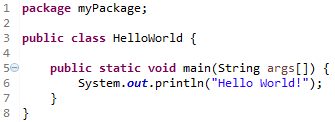
\includegraphics[width=300pt]{Images/Package}
	\caption{Use of a non-default package; please don't do this}
	\label{fig:package}
\end{figure}

\subsection{Types of Input}
In this subject, we make a distinction between two types of input: Command line arguments, and User input.

\subsubsection{Command Line}
Lab tasks that require the use of command line arguments will say explicitly that your program should accept command line arguments, or data will come from the command line''.\\

When writing your code to solve these problems, \textbf{do not} use a Scanner. All inputs will be provided via the command line, meaning (if you are using an IDE, like Eclipse or NetBeans) you must set the run configurations of your project to provide arguments.\\

\begin{figure}[!h]
	\centering
	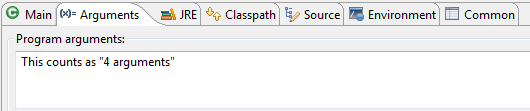
\includegraphics[width=300pt]{Images/CommandLineEclipse}
	\caption{Inputting data using the command line in Eclipse}
	\label{fig:commandLineEclipse}
\end{figure}

To do so in Eclipse, click on the ``Run'' menu, then ``Run Configurations''. On the following window, click arguments, and you will arrive at the window shown in Figure \ref{fig:commandLineEclipse}. For NetBeans, click on the ``Run'' menu, then ``Set project Configuration $\rightarrow$ Customize...'' to arrive at the window shown in Figure \ref{fig:commandLineNetBeans}\\

\begin{figure}[!h]
	\centering
	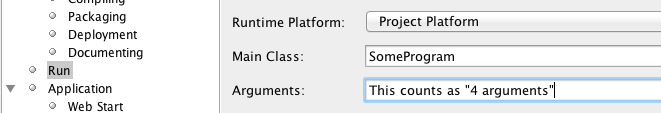
\includegraphics[width=300pt]{Images/CommandLineNetBeans}
	\caption{Inputting data using the command line in NetBeans}
	\label{fig:commandLineNetBeans}
\end{figure}

Each distinct word on the command line is treated as a separate input and will appear as a distinct element in the \verb|args| variable. The exception to this is words within quotation marks; all words within quotes are treated as a single string. For the example input in Figure \ref{fig:commandLineNetBeans}, \verb|args| will look as follows:
\begin{description}
	\setlength{\itemsep}{-.3em}
	\item[args[0]] = "This"
	\item[args[1]] = "counts"
	\item[args[2]] = "as"
	\item[args[3]] = "4 arguments"
\end{description}

\subsubsection{User Input}
Lab tasks that require you to print a prompt or read input \textbf{must} be written using a Scanner; there will be no input from the command line. For these tasks, you must use \verb|nextLine()|, \verb|nextInt()|, and other Scanner methods to get input from the ``user''.\\

When submitting programs that make use of Scanner for assessed labs, there is obviously no one on the other end typing input for you. When using a Scanner, input may also be provided through a text file. To your code, there is no difference in either method; you must use the Scanner to read input.

\section{Submitting from home}
\label{sec1}
If you are submitting using a University lab computer, skip straight to section \ref{sec2}.\\

Before submitting from home, you \textbf{must} log in to one of the University lab computers \textbf{at least} once, or you will not be able to access the servers or copy files to them. To submit from home, you first need to download the University's VPN service, which you can get \href{https://its.unimelb.edu.au/help/networks-access/networks-internet/vpn/installing-anyconnect}{here}. Once on the page, click the ``student'' link, and use your student login to continue to the screen shown in Figure \ref{fig:ciscoDownload}. After the site has verified your system, an installer will download to your computer to install the VPN software.\\

\begin{figure}[!h]
	\centering
	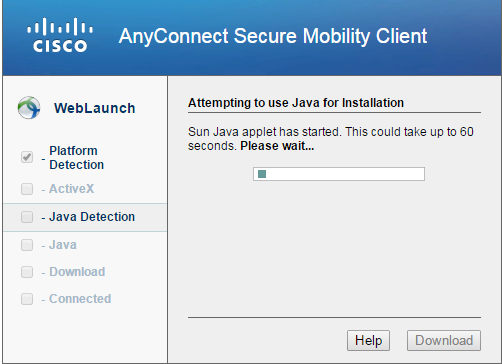
\includegraphics[width=200pt]{Images/CiscoDownload}
	\caption{Cisco AnyConnect download screen}
	\label{fig:ciscoDownload}
\end{figure}

When you run Cisco AnyConnect, you will see the screen shown in Figure \ref{fig:ciscoRun}. Click connect, and enter your student login information to connect to the university servers. If you are successful, you will see the Cisco symbol in your system tray (on Windows). You can now proceed with section \ref{sec2}.

\begin{figure}[!h]
	\centering
	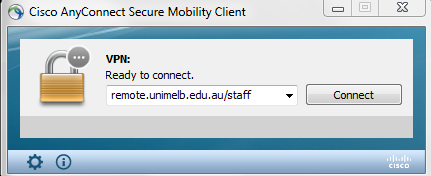
\includegraphics[width=200pt]{Images/Cisco}
	\caption{Cisco AnyConnect run screen}
	\label{fig:ciscoRun}
\end{figure}

\section{Transferring files to server}
\label{sec2}
If you are submitting using a lab computer, make sure your files are stored on the H: drive; if they are anywhere else, you will not be able to find them. In this case, skip to section \ref{sec3}.\\

In order to submit your assignment, your \textit{.java} files \underline{must be on the university servers}. The easiest way is to use a file transfer program, such as WinSCP, FileZilla, or MobaXterm. These instructions show WinSCP, but should be almost identical for other programs.\\

When you launch WinSCP you will get the screen shown in Figure \ref{fig:WinSCPLogin}. In some cases (like in FileZilla) the port number will be empty; make sure to always use port 22. Use your university login to connect to either
\begin{center}
\verb'nutmeg.eng.unimelb.edu.au'

\verb'dimefox.eng.unimelb.edu.au'
\end{center}

\begin{figure}[!h]
	\centering
	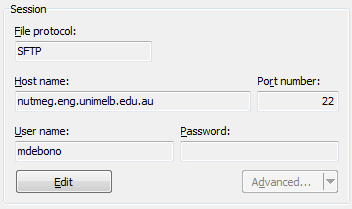
\includegraphics[width=200pt]{Images/WinSCPLogin}
	\caption{WinSCP login screen}
	\label{fig:WinSCPLogin}
\end{figure}

After connecting you will see the screen shown in Figure \ref{fig:WinSCPFiles}. The left hand explorer window shows files on your local computer, the right hand side are files on the University servers. To transfer your files, simply locate them on the left side and drag them to the right. Your files are now on the server and should appear on the right hand explorer window; you can submit!

\begin{figure}[!h]
	\centering
	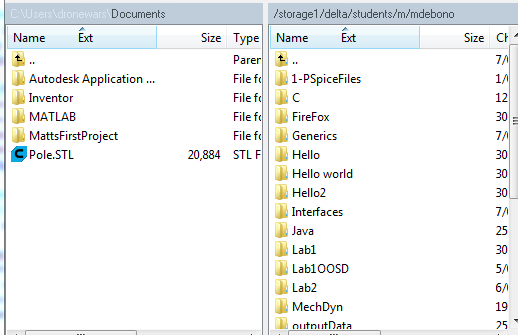
\includegraphics[width=300pt]{Images/WinSCPFiles}
	\caption{WinSCP file browser}
	\label{fig:WinSCPFiles}
\end{figure}

\section{Submitting your assignment}
\label{sec3}
\underline{You must perform this step in order to get marks}. Transferring your files to the server is \underline{not} the same as submitting your files.\\

To submit your files, you need to use a terminal program. Mac users may use the inbuilt terminal, but Windows users must download a program capable of SSH connections; these instructions will use Putty.\\

To connect using the Mac terminal, simply type
\begin{center}
\verb'ssh "your username here"@nutmeg.eng.unimelb.edu.au' or\\
\verb'ssh "your username here"@dimefox.eng.unimelb.edu.au'\\
\end{center}
(without the quotation marks), and follow the instructions below. When you launch Putty, you will see a similar screen to using WinSCP; use either \verb'nutmeg' or \verb'dimefox' to connect to the servers, and again make sure to use port 22, as in Figure \ref{fig:Putty}. Please note that even though no characters appear on the screen, \underline{you are typing your password in}.\\

\begin{figure}[!h]
	\centering
	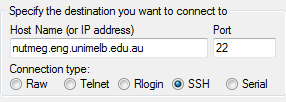
\includegraphics[width=200pt]{Images/Putty}
	\caption{Putty login screen}
	\label{fig:Putty}
\end{figure}

Once you have connected, you will see the black terminal screen. Before you submit, type \textbf{ls} to \textbf{list} the files in your current directory. As you can see in Figure \ref{fig:ls}, there are no \textit{.java} files but there are directories, coloured in blue. If this is the case, use \textbf{cd} to \textbf{change directory}, and move down into the folder where you put your files. For example, if you put your files in the \textbf{Lab1} folder, you would type \textbf{cd Lab1/} to move into that folder. Continue using \textbf{ls} and \textbf{cd} until you have found your files.\\

\begin{figure}[!h]
	\centering
	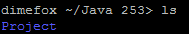
\includegraphics[width=200pt]{Images/ls}
	\caption{Putty files list; notice there are no \textit{.java} files}
	\label{fig:ls}
\end{figure}

\newpage
Finally, it's submission time! You can use the \verb'submit' command to submit your assignment, which looks like\\

\verb'submit mySubject myAssessment myFiles'\\

For lab 1, your submit command will be\\

\verb'submit COMP90041 lab1 Welcome.java Circle.java'\\

Note: COMP90041 is \underline{not} a folder in your H: drive, it is the subject you are submitting for. If you put your files in a folder named COMP90041, but cannot see them when you type \textbf{ls}, then you have not followed the instructions above and won't be able to submit. If you receive an error that says \textit{submit: command not found}, then you need to update your path to be able to find submit; just type in

\verb'PATH=/usr/local/bin/:'\$\verb'PATH'\\

Finally, make sure you submit all required files at the same time; only your last submission is recorded, so if you only submit one file, and try to submit another file in the next submission, this will not work. Submit all files together!

\section{Getting feedback}
\label{sec4}
The final step in submitting your assessed labs is getting your feedback, and checking your marks. Each of the assessed labs is marked almost instantly, so don't forget this step! We won't be sympathetic to people who send us emails after the due date, asking why they didn't get full marks \smiley{} \\

To get your feedback, in Putty or your Mac terminal, type\\

\verb'verify COMP90041 lab1'\\

Verify will also print out your code, so to make it more readable you can use either of the following. The first will print one screenful of text at a time; you can use \textit{spacebar} to go to the next screen, \textit{b} to go back, and \textit{h} for help. The second version will print everything to ``myFeedback.txt'', which you can view on a lab computer, or by transferring back to your computer.\\

\verb'verify COMP90041 lab1 | less'

\verb'verify COMP90041 lab1 > myFeedback.txt'\\

Finally, when viewing verify, you may see a \textbf{diff} message, which shows you where your output has differed from the expected output, but only if there are differences detected. As mentioned above, if you have a package statement at the top of your \textit{.java} file, your code \underline{will not} execute correctly, and will not give any output.\\

In the \textbf{diff statement}, lines with a minus sign (-) are the correct answer. Lines with a plus (+) sign are lines printed by your code. Compare the plus and minus lines to identify where you may have errors. If you do not have any plus lines, you have not payed attention, and you have a package statement in your \textit{.java} file. The most common \textbf{diff} error to receive is ``no newline character at end of output''. To fix this, make sure that your final print statement is either System.out.println, or you place ``$\backslash$n'' at the end of the string.\\

Congratulations on submitting your assignment! Good luck!


\end{document}
